\documentclass{article}
\usepackage[minionint,mathlf,textlf]{MinionPro} % To gussy up a bit
\usepackage[margin=1in]{geometry}
\usepackage{graphicx} % For .eps inclusion
%\usepackage{indentfirst} % Controls indentation
\usepackage[compact]{titlesec} % For regulating spacing before section titles
\usepackage{adjustbox} % For vertically-aligned side-by-side minipages
\usepackage{array, mathrsfs, mathrsfs, mhchem, amsmath} % For centering of tabulars with text-wrapping columns
\usepackage{hyperref, chemfig}
\usepackage{subfigure}
\newcommand{\Lapl}{\mathscr{L}}

\pagenumbering{gobble} 
\setlength\parindent{0 cm}
\begin{document}
\large

\section*{Introduction to regeneration}

In our last lecture, we saw many examples of development where an initial continuous gradient is ``read out" into increasingly-refined, discrete territories to pattern an embryonic axis. We focused mainly on anterioposterior axis formation in Drosophila and its origin in, for example, the gradient of Bicoid protein created due to inhomogeneity in the cytoplasmic localization of the mRNA during oogenesis. Proportionality between embryonic regions and their identity depended on the amplitude and shape of this gradient: we discussed several mechanisms which an embryo might use to make such a gradient robust to variation in embryo length and mRNA number (and to read out position on a variable gradient more accurately).\\

Variation in egg length and mRNA number aside, we might envy the organism'ss significant control over the initial conditions in embryogenesis when we compare it to another developmental process: regeneration. The ability to regenerate is highly variable across taxa, though there are obvious potential advantages to recovery after injury. Having observed fruit fly development from the embryogenesis perspective, it is easy to ``understand" why the fruit fly cannot regrow a new head, and probably tempting to conclude that a complex developmental program cannot be encoded reliably in a way that permits regeneration. Yet wound healing and regeneration are commonplace in higher plants, and many metazoans show remarkable though incomplete regenerative abilities. Regeneration may be a simple matter when development is favorably organized.\\

As a simple example, consider the brown alga genus \textit{Fucus}. The first axis apparent in the embryo distinguishes the rhizoid (a root- or holdfast-like structure) from the stipe and blades (``stem" and ``leaves"). The cue for establishing this axis appears to be simply the direction of incident light and the production of reactive oxygen species, both of which are a consequence of the orientation in which the zygote lands on a substrate. This environmental inhomogeneity is reliably present, so there is no need for a maternal factor to pattern this axis\footnote{Reactive oxygen species also pattern the oral-aboral axis in sea urchin larvae, which at this stage may be free-floating. It has been argued that random differences in mitochondrial distribution during early cleavage are sufficient to pattern the axis in this case.}. It may not surprise you to learn that \textit{Fucus} species are capable of regeneration.

\begin{center}
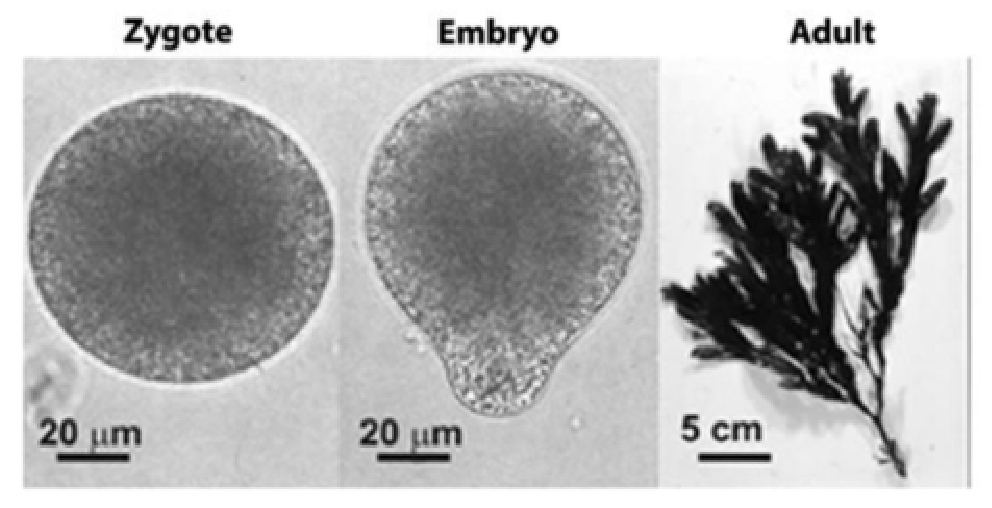
\includegraphics[width=0.6\textwidth]{fucus.pdf}
\end{center}

A common theme in regenerating organisms is that one or more cell types possesses the ability to reproduce indefinitely, whether through maintenance of a pluripotent state or through ``de-differentiation" in response to injury. A theoretical danger of this approach is that, through mutation, such cells may lose growth or differentiation regulation to become cancerous. However, organisms such as urodeles and planaria show no evidence of increased risk for tumor formation: indeed, the axolotl is over 1000 times more resistant to cancer than the average mammal. It remains an open question what features of regeneration systems minimize this risk.

\section*{Epimorphosis in teleosts and urodeles}

Some bony fish and most salamanders (a subgroup of amphibians also known as urodeles) can regenerate lost limbs. This capacity is not shared with the amniotes: for example, humans are capable of regenerating only the tips of their fingers, and even then, only in youth. There is insufficient evidence to claim that regenerative capacity was present in a common ancestor but ``lost" in most lineages, rather than gained twice independently in the fish and salamanders.

\begin{center}
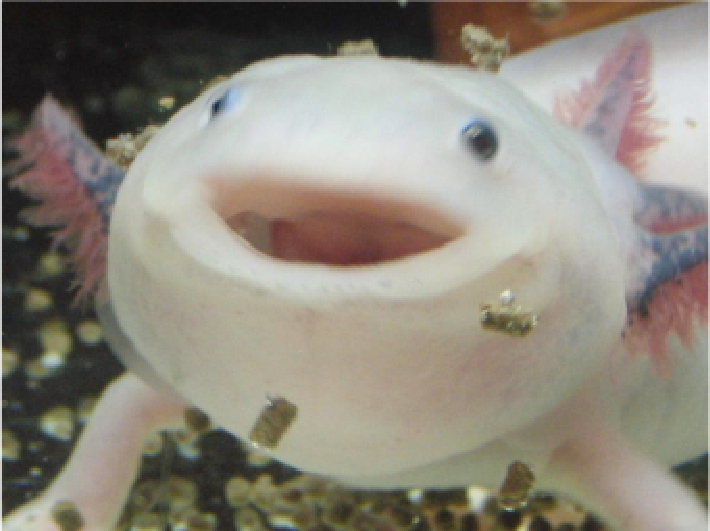
\includegraphics[width=0.4\textwidth]{axolotl.pdf}
\end{center}

The model organism for salamander limb regeneration is the axolotl (genus \textit{Ambystoma}), a particularly ugly  creature with distinctive external gill stalks. After limb loss, cells dedifferentiate at the site of injury and proliferate to form a blastema, which grows outward until the whole limb has been replaced. (Only osteoclasts are thought to arrive by migration: these cells help degrade bone at the site of injury.)

\begin{center}
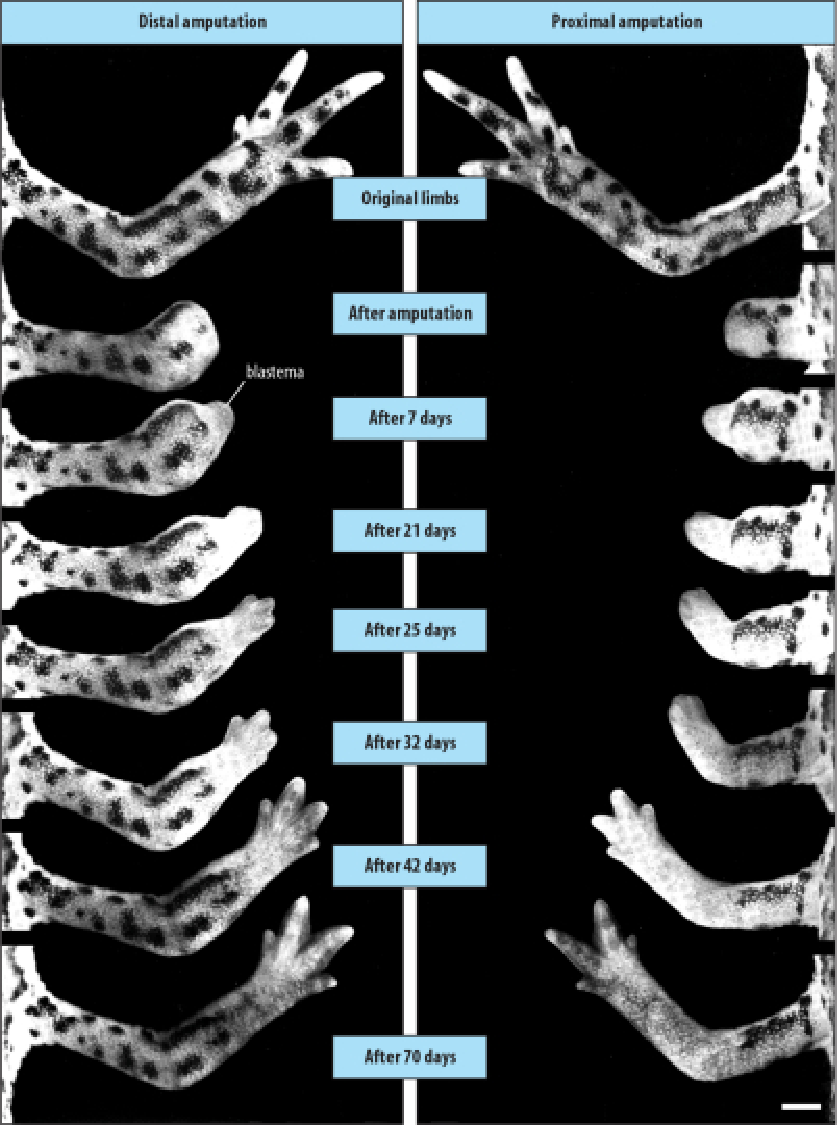
\includegraphics[width=0.4\textwidth]{amphibian_limb.pdf}
\end{center}


The mechanism by which dedifferentiation occurs remains of great interest because of the medical importance of replacing lost cell populations with differentiated cells genetically identical to the patient. A long-sought approach to such therapies involves producing a genetically-identical pluripotent cell population via somatic cell nuclear transfer or induced pluripotency, performing a genetic modification if necessary, then causing these cells to differentiate into the desired type either by replicating the natural differentiation cues in the growth media or by forcing expression of cell type-specific genes (particularly, of transcription factors that serve as ``master regulators"). These methods typically risk failure of complete differentiation (and consequent unregulated growth) of replacement cells. Axolotl blastema dedifferentiation, by contrast, appears naturally self-limiting, in that even when cultured independently, blastemal cells will redifferentiate.

\section*{Regeneration in planaria}

\begin{center}
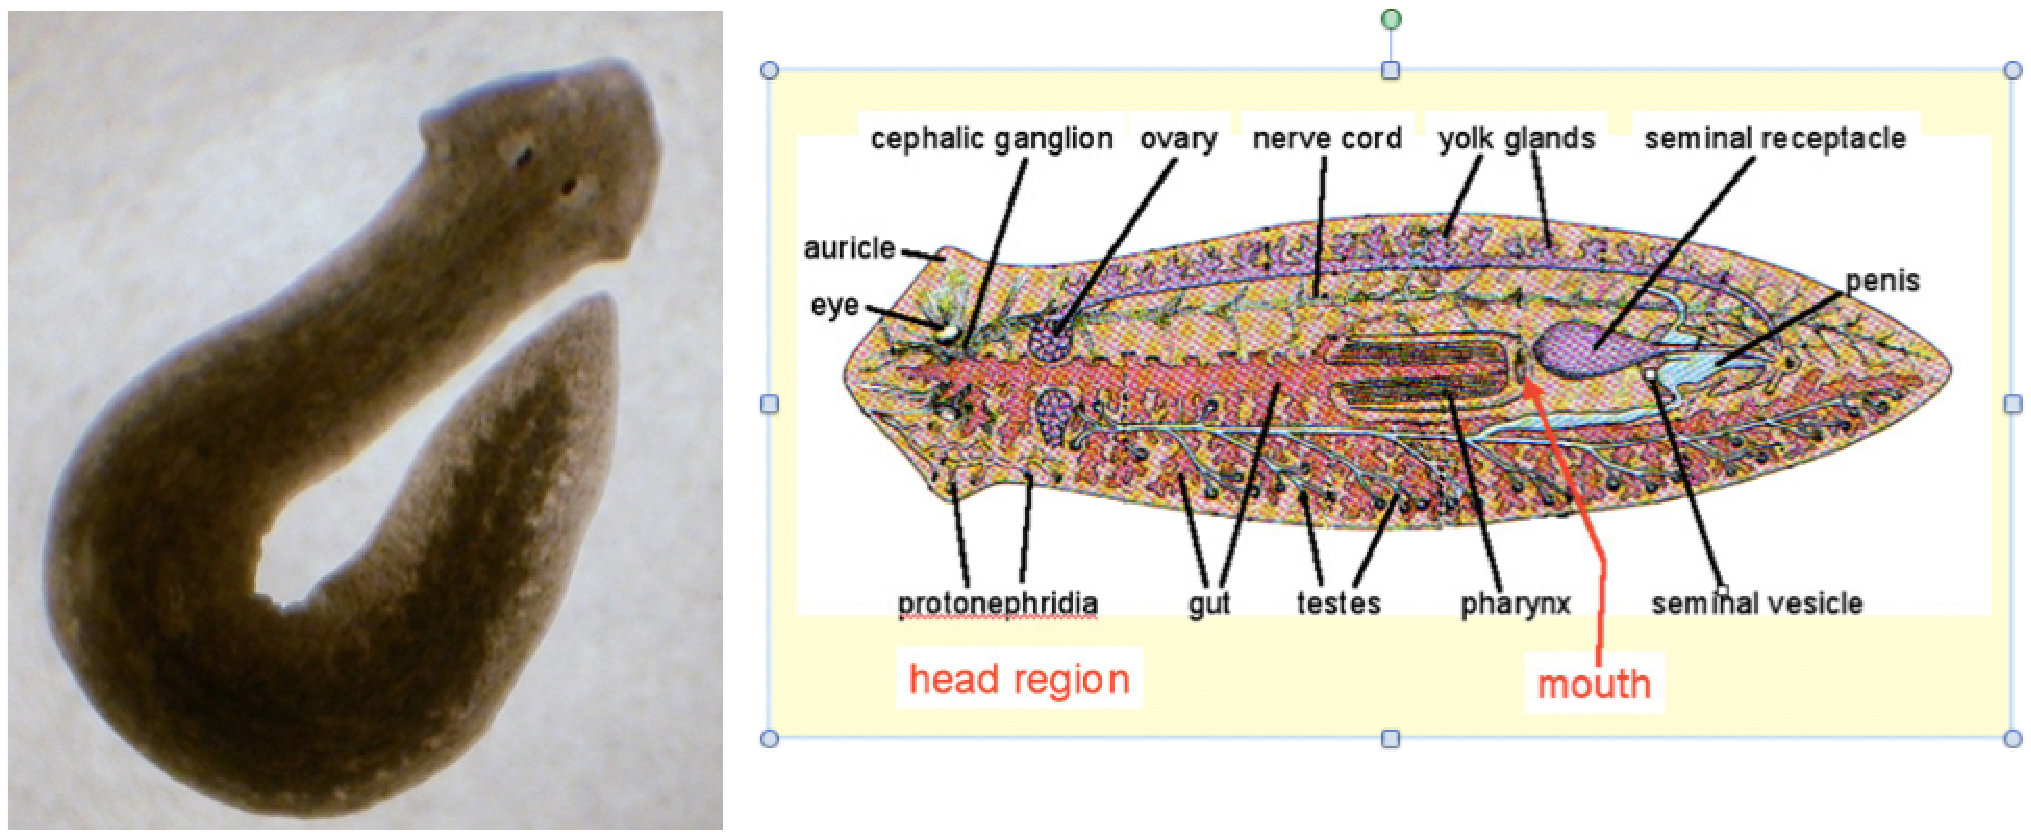
\includegraphics[width=0.8\textwidth]{planaria_anatomy.pdf}
\end{center}

The flatworm \textit{Schmidtea mediterranea} can regenerate any tissue following a sordid array of injuries. Planarians make dramatic recoveries following cuts perpendicular to the anterioposterior and mediolateral axes\footnote{Slicing in the plane perpendicular to the dorsoventral axis would likely cause excessive injury, and apparently has not been attempted.}, and fissure wounds.

\begin{center}
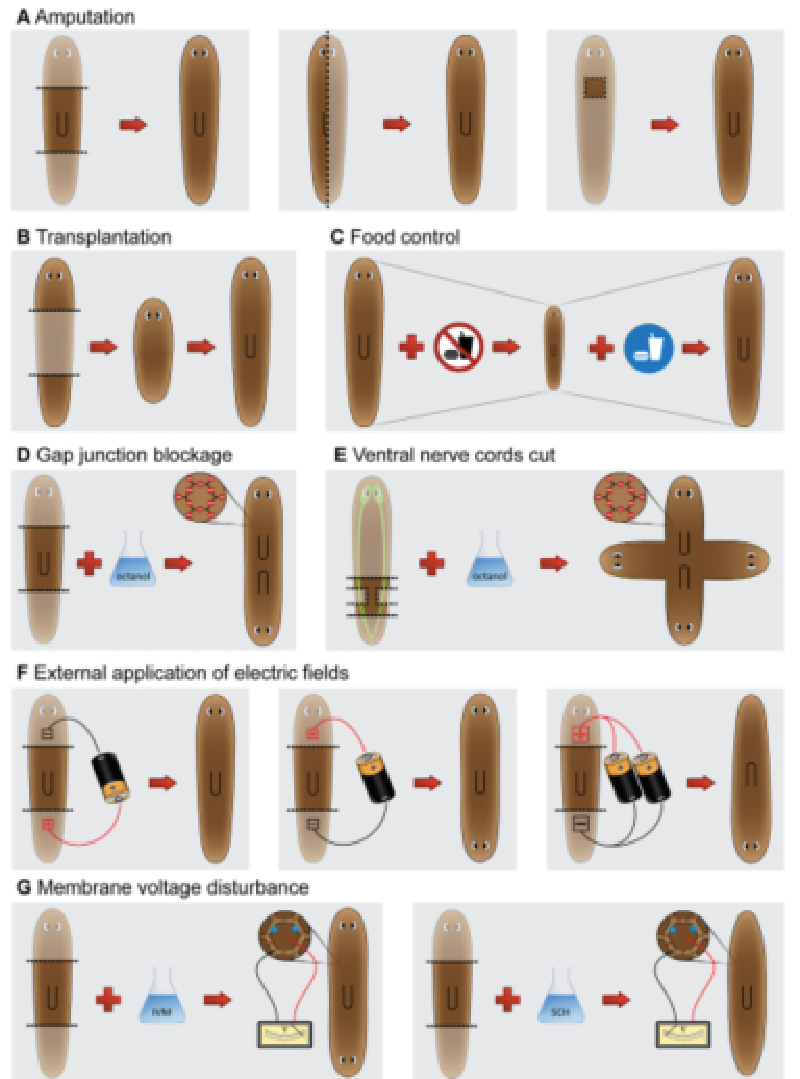
\includegraphics[width=0.5\textwidth]{injuries.pdf}
\end{center}

\begin{center}
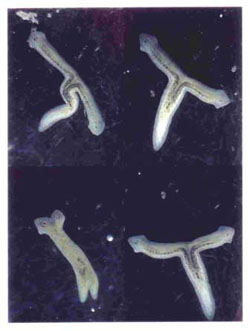
\includegraphics[width=0.3\textwidth]{planaria_twoheads.jpg} \hfill 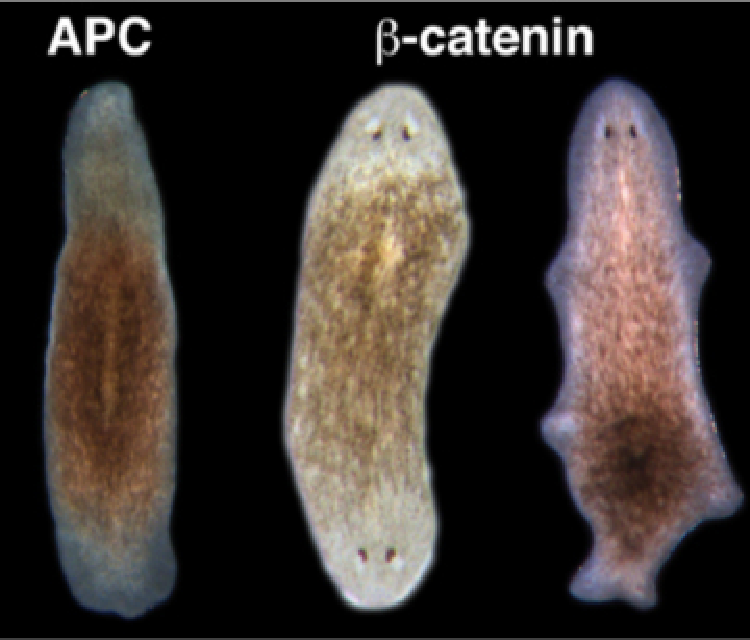
\includegraphics[width=0.45\textwidth]{heads.pdf}
\end{center}

Despite an outwardly simple appearance, these planarians possess many organ systems including a ladder-like nervous system with central ganglia, reproductive and excretory systems, musculature, a gastrointestinal cavity and pharynx, eyespots, and chemosensory organs called auricles (positioned at the side tips of their diamond-shaped heads) -- anatomical complexity that makes their regenerative potential all the more extraordinary.\\

Like urodeles, \textit{S. mediterranea} regenerates through proliferation of undifferentiated cells whose descendants differentiate into the missing tissues. Unlike the urodeles, however, these undifferentiated cells are always present in planaria, where they make up an astonishing 20-30\% of all cells in the body. These totipotent cells called (sigma) neoblasts: normally they replace cells in normal tissue turnover and produce new cells as the organism gorws, but following injury, they migrate to the wound and proliferate to form a blastema that gives rise to the regenerated tissue (von Wolfswinkel et al., 2014). After an amputation, epithelial cells close the wound within about one hour, and neoblasts near the site (or in some species, throughout the flatworm) proceed more rapidly through mitosis. Neoblasts accumulate just behind the newly-formed epithelium through a combination of migration and proliferation for about four days. Molecular markers of the regenerating body parts can be detected at this time: full regeneration and proportionality-restoring growth can take several weeks.

\begin{center}
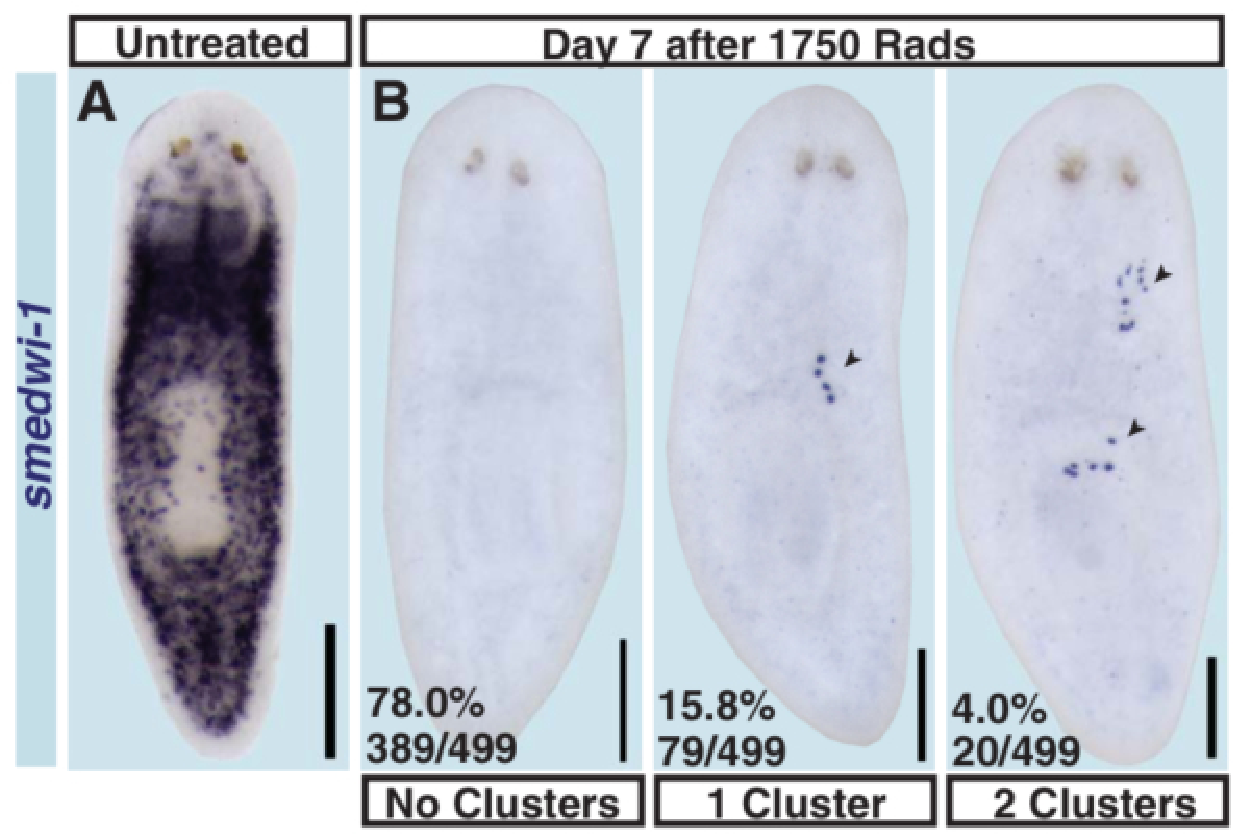
\includegraphics[width=0.5\textwidth]{neoblast.pdf}
\end{center}

The proliferative capacity of neoblasts is such that a single cell can restore growth and regenerative capacity to an irradiated animal (Wagner et al., 2011). The neoblast forms a significant colony but cannot proliferate and migrate throughout the decaying host in time to maintain its original size: as a result, about two weeks after irradiation the host begins to regress, apparently leaving only the region which has been populated by the neoblast clone, from which the flatworm then regenerates. In this rather unnatural context (which bears resemblance nonetheless to dedifferentiatiion and bone dissolution in amphibian limb regeneration) the planarian must \textit{reculer pour mieux sauter} (Needham 1961).

\begin{center}
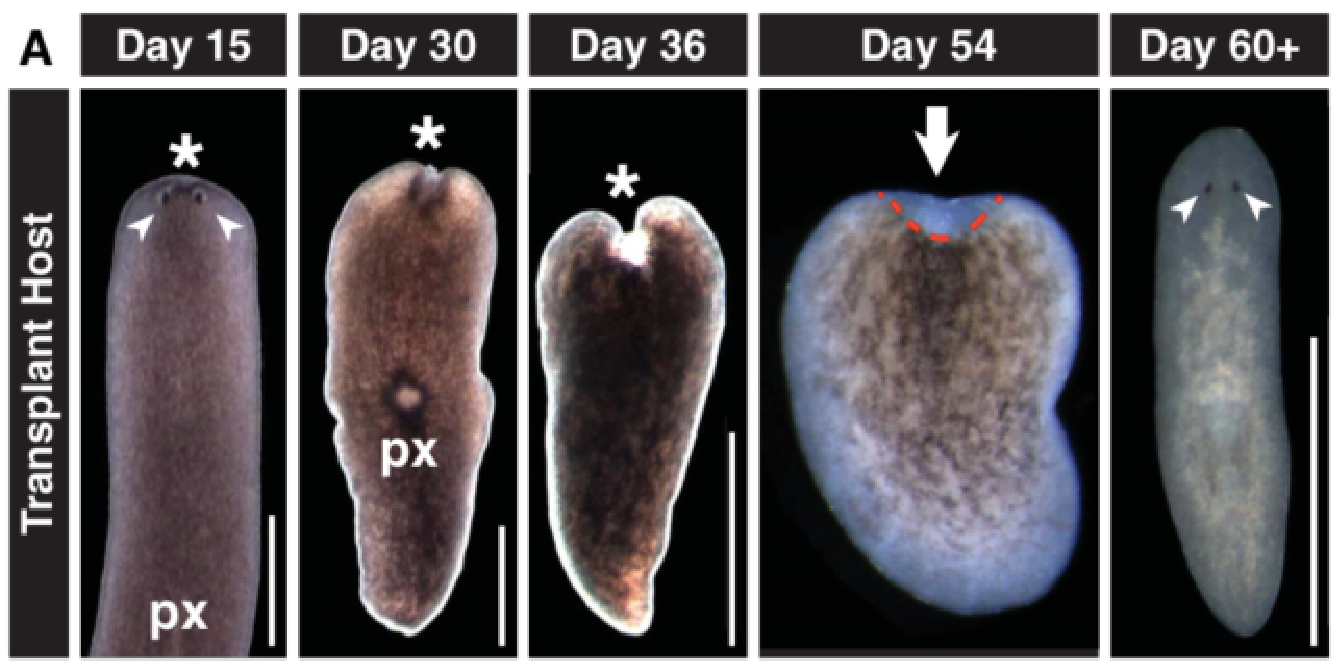
\includegraphics[width=0.6\textwidth]{regression.pdf}
\end{center}

Neoblasts rely on cells near the site of injury to provide spatial cues that indicate which tissue is missing at the site of the blastema. A challenge exists in planarian regeneration that is not evident in urodele limb regeneration: remembering axial polarity. The limb regeneration always occurs in the proximal to distal direction: the severed limb does not regenerate a body. However, the planarian's head may regenerate its body, or vice versa: the planarian blastema therefore needs to know not only where it is but also in which direction it is growing.

\begin{center}
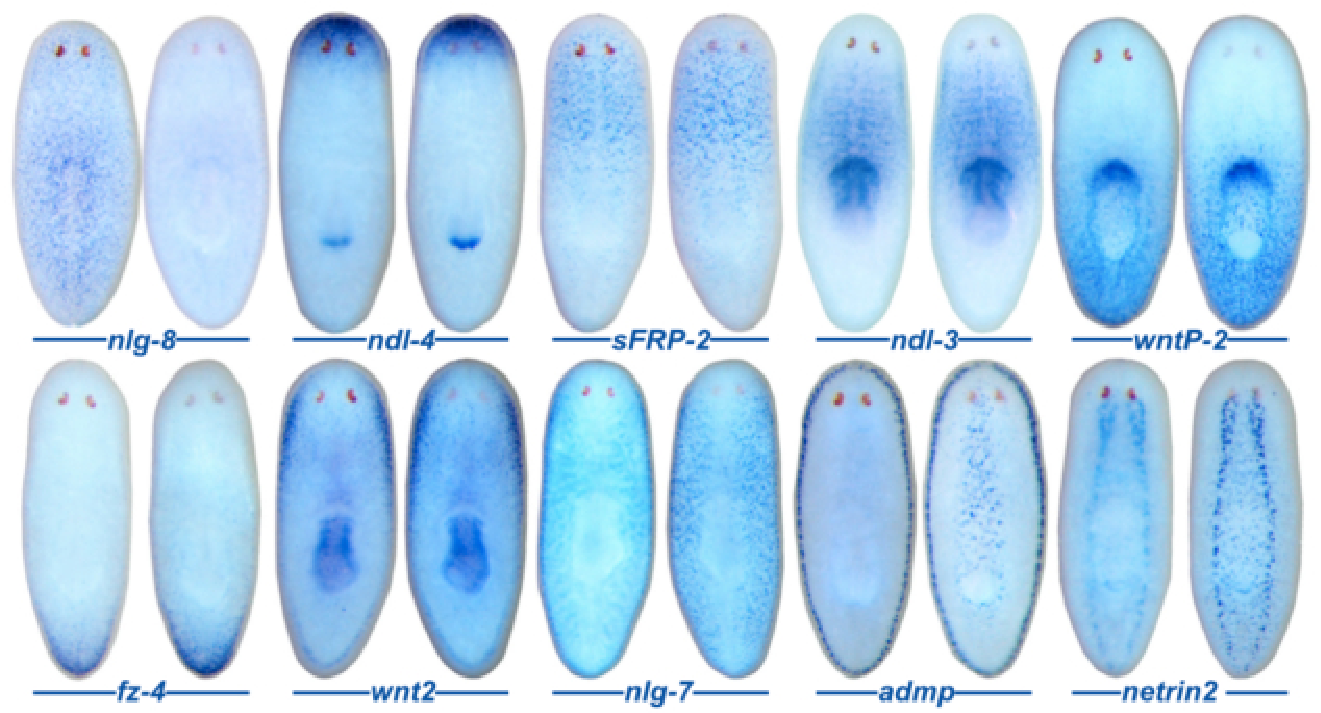
\includegraphics[width=0.6\textwidth]{pcg.pdf}
\end{center}

Neighboring muscle cells provide positional cues to neoblasts (Witchley et al., 2013). Extracellular signaling molecules like Wnt1 (a posterior pole cue), Notum (a Wnt inhibitor expressed at the anterior pole), and Bmp4 (a mediodorsal cue) are expressed by muscle cells depending on their relative position and thus act as a form of positional memory. Four days following injury, however, muscle cells begin to express positional cues appropriate to their new relative position within the embryo. This dynamic change in positional cues may be important for instructing neoblasts on the appropriate polarity for the blastema. (In the case of Notum expression at anterior-facing wounds, it may also be necessary to inhibit posterior identity signals in the new tissue.) Another opportunity for neoblasts to sense the polarity of the tissue is afforded by their migration to the site of injury, which would expose the cell to changes in the morphogen gradient, though I am unaware of any evidence that neoblasts make use of this clue.

\section*{Maintenance of a stem cell niche}

On a less grand scale, the principle at work in planaria -- maintenance of a stem cell population which can give rise to differentiated cell types -- is used for tissue maintenance in many contexts. For example, stem cells within intestinal crypts continuously produces more epithelial cells to replenish the microvilli sloughed away by passing material. The rates of proliferation and differentiation of these stem cells is expected to be tightly linked to avoid complete loss of the stem cell population through differentiation.\\

The essential problem is that one-way conversion can lead to loss of the stem cell type. If the population is assumed to be perfectly mixed, then a deterministic model for the growth of the stem cell $a$ and differentiated cell $b$ populations follows (time here is measured in units of the division time of the stem cell population):
\[ \frac{d}{dt} \begin{pmatrix} a \\ b \end{pmatrix} = \frac{d}{dt} \begin{pmatrix} 1 - \mu & 0 \\ \mu & 1 + s \end{pmatrix}  \implies \begin{pmatrix} a(t) \\ b(t) \end{pmatrix} = c_1 \begin{pmatrix} s - \mu \\ \mu \end{pmatrix} e^{(1-\mu)t} + c_2 \begin{pmatrix} 0 \\ 1 \end{pmatrix} e^{(1-s)t} \]
where $s$ is the growth rate difference of differentiated vs. stem cells and $\mu$ is the conversion rate. (The system was solved by determining the eigenvalues and corresponding eigenvectors, just as you did when analyzing linear systems.) It is easily seen that if $s$ is greater than $\mu$, at long times the stem cell population will decay to nothing. By reexpressing this system with $f=a/(a+b)$, the expected rate of change in the fraction of stem cells in the population can be found to be:
\[ \frac{df}{dt} = sf(1-f) - \mu f \]
In this form we can more easily model the stochastic effects in small populations. Just as you saw in the last homework, when stochastic fluctuations are permitted, at very long times it is expected that the stem cell population will be lost, though a nonzero $f$ is stable in the deterministic system for any $\mu > s$. (This problem is equivalent to that of mutation-selection balance in well-mixed populations.)\\

Another disadvantage of maintaining a stem cell population arises from the fact that organisms normally are not well-mixed. The fewer effective dimensions in which cells proliferate, the larger the probability that the stem cell lineage will be lost entirely (Lavrentovich 2015ab; Lavrentovich et al., 2013).

\section*{Morphallaxis in hydra}

Of the serpent Hydra of Greek mythology, it was said, ``Cut off one head, two more shall take its place." Real hydra are typically half an inch in length and possess no true ``head," but rather a collection of tentacles extending from a tubular body column which attaches to surfaces through a specialized ``foot." (The positioning of these tentacles along the ring-like body was an original motivating question in Alan Turing's 1952 paper on pattern formation, which we will cover in our next lecture.) What real hydra do share with their mythological counterpart is the ability to regenerate and an apparent immortality (that is, the failure of an individual hydra to senesce).

\begin{center}
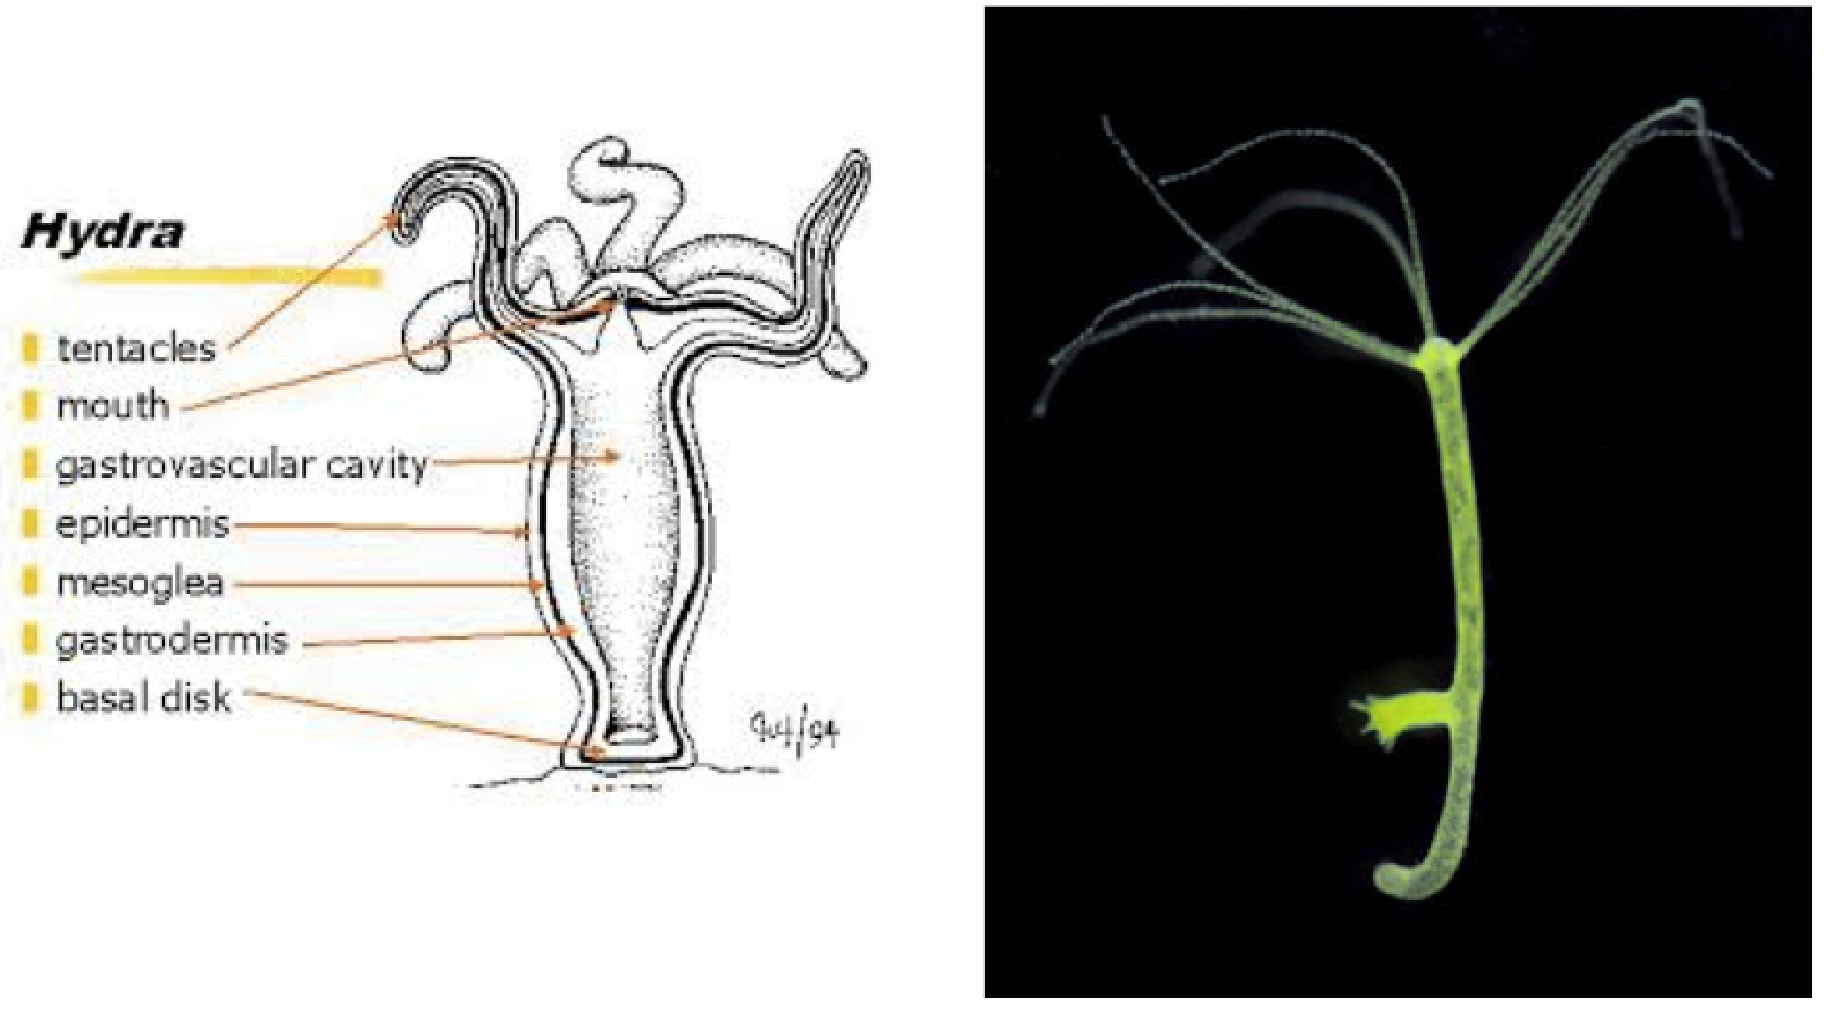
\includegraphics[width=0.8\textwidth]{hydra_anatomy.pdf}
\end{center}

[Draw phylogenetic tree of metazoans at board]. Unlike their close relatives the jellyfish, with the exception of their free-swimming sperm, hydra remain attached to a substrate throughout their life cycle. Hydra are diploblastic (do not possess a true mesoderm) and possess some specialized cell types including a central digestive cavity, a neural net, specialized stinging cells alled cnidocytes, differentiated gonads, and mesoglea. All of these tissues and cell types must be regenerated both following injury and during normal growth, to prevent senescence.\\

Hydra can regenerate both head and foot in the two fragments formed by decapitation and so, like flatworms, must maintain positional and directional cues during regeneration. Some specifics of the systems that provide this information are already established (see e.g. Chera et al., 2009). Unlike planaria, regeneration of the head in hydra can be achieved without cell proliferation to produce two hydra half the size of the original. (Cell proliferation does normally occur but is not contribute as substantially as it does in epimorphosis.)

\begin{center}
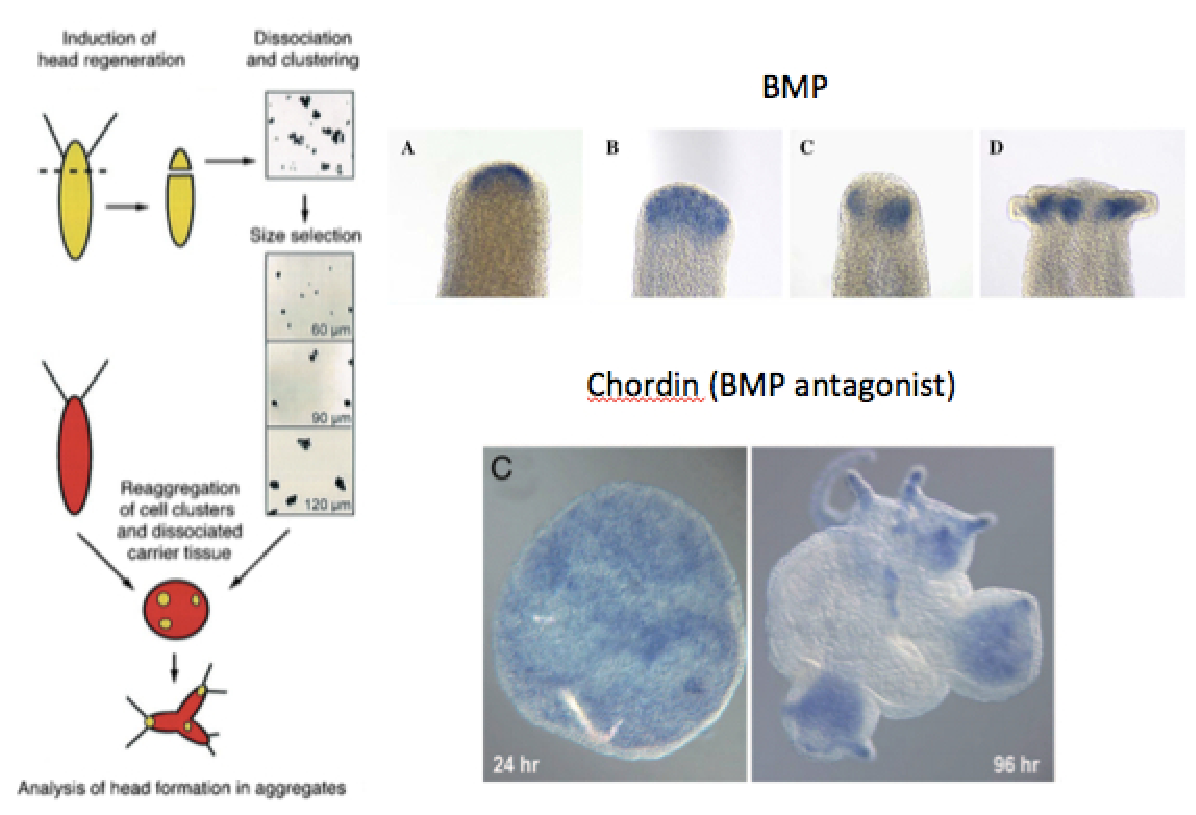
\includegraphics[width=0.8\textwidth]{reconstituion.pdf}
\end{center}

Another striking feature of some hydra and sponges is that a functioning organism can be reconstituted from individual cells. When the cells of these organisms are dissociated and mixed back together, they self-organize within 2-3 days to form regularly-spaced ``heads" which organize surrounding cells into corresponding bodies. Five to fifteen epithelial cells can suffice to form a ``head-organizing center" which represses the formation of other heads nearby\footnote{The traditional name for this region is the hypostome: it was the first organizing center discovered (even preceding Spemann's organizer).}. Unlike the lateral inhibition examples which we have discussed so far, these organizing centers consist of multiple cells, suggesting a community effect. This pattern is thought to reflect two diffusing signals: the first, a short-range activator; and the second, a longer-range inhibitor of head formation. The two signals involved are orthologs of Chordin (a BMP inhibitor) and BMP (Reinhardt et al., 2004 and Rentzsch et al., 2007). You may find it surprising that a ligand and its own inhibitor are both produced in the same location: the possible purpose of this will become apparent in our next lecture on Turing patterns.

\section*{Responses to in-class questions}

Following up on the exponential scaling of gradients we discussed last time, it was asked how a comparison between two oppositely-oriented exponential gradients can lead to scaling of axial patterning. McHale et al. (2006) consider first the case of two non-interacting transcription factors $A$ and $B$ which each form exponential gradients from opposite poles (similar to Bicoid and Nanos protein). They imagine a target gene in which the binding sites for the two transcription factors overlap: the gene is only expressed when $A$ is bound at its site and thus has recruited RNA polymerase:  the probability of this is taken to be some function $f(A,B)$. Assuming that the probability of $A$ not being bound is much larger than the alternative, $f(A,B) \approx P_{on}/P_{off}$, McHale et al. show that $f(A,B) = f(A/B)$. They further show that \textit{at exactly one point}, a fractional position of the total length $L$ can be determined independently of $L$ as a function of $A/B$. The scaling nearby is not perfect but  is reasonably good, e.g. $\leq 5$\% error over the middle forty percent of the length under certain conditions. Later in the same paper they consider a mutual annihilation model where the region of accurate scaling is substantially extended.\\

Other examples of activator-inhibitor pairs besides Chordin/Noggin and BMP include sFRP \& Wnt and Sprouty \& FGF. (Nodal and Decapentaplegic are homologs of BMP.) Chordin, Noggin, and sFRP bind to their corresponding signaling proteins to prevent them from activing cell surface receptors. Dickkopf and Sprouty instead work by inhibiting the receptor.

\end{document}